\documentclass[docid=2020]{comp_test1}
\begin{document}
\renewcommand\thesubsubsection{\thesubsection.\arabic{subsubsection}}
\setcounter{chapter}{2020}
\exam{2020 Test 1}

\examgroup{Lexical and Syntactic Analysis}

The CFG (Context-Free Grammar) G1 below represents a grammar of a simple programming language.

~

\begin{minipage}[t]{0.44\textwidth}
    Some of the Tokens for G1:
    
    \begin{itemize}[wide, noitemsep, label={}]
        \item \texttt{REG = \$[0-9][0-9]}
        \item \texttt{IF = if}
        \item \texttt{GOTO = goto}
        \item \texttt{CMP = == | < | > | <= | >= | !=}
        \item \texttt{CONST = [0-9]+}
        \item \texttt{OP = + | -| * | /}
        \item \texttt{LABEL= [a-zA-Z][a-zA-Z]*}
    \end{itemize}
\end{minipage}
\begin{minipage}[t]{0.54\textwidth}
    Grammar G1:
    
    \begin{enumerate}[wide, noitemsep]
        \item \texttt{S → Stmt (Stmt)*}
        \item \texttt{Stmt → LABEL: | Assign | If| GOTO LABEL;}
        \item \texttt{Assign → Lhs= Operand (OP Operand)?;}
        \item \texttt{Operand →REG | CONST | Mem}
        \item \texttt{If → IF Cond GOTO LABEL}
        \item \texttt{Cond → Operand CMP Operand }
        \item \texttt{Lhs → REG| Mem}
        \item \texttt{Mem → “M["Operand“]”}
    \end{enumerate}
\end{minipage}

\question
Write the chain of the first 10 tokens resultant from the lexical analysis for Code1 below;

\begin{lstlisting}[caption=Code1]
    $2=0;
L2:
    if $2 >= 100 goto L1
    $3 = 4*$2;
    $4 = $1+$3;
    M[$4] = 0;
    $2 = $2+1;
    goto L2;
L1:
\end{lstlisting}

\ansseparator

\noindent
\texttt{REG(\$2)}, \texttt{T1(=)}, \texttt{CONST(0)}, \texttt{T2(;)}, \texttt{LABEL(L)}, \texttt{CONST(2)}, \texttt{T3(:)}, \texttt{IF}, \texttt{REG(\$2)}, \texttt{CMP(>=)}

\question
Give the \textit{First} and \textit{Follow} sets for the grammar variables: \textit{Assign}, \textit{Lhs}, and \textit{If};

\ansseparator

\vspace{-2.0em}
\begin{alignat*}{5}
    & First (Assign) &&= \{ \texttt{REG}, \texttt{"M["} \} && ~~~~~~~~~~ && Follow(Assign) &&= \{ \texttt{LABEL}, \texttt{REG}, \texttt{"M["}, \texttt{IF}, \texttt{GOTO} \} \\
    & First (Lhs)    &&= \{ \texttt{REG}, \texttt{"M["} \} && ~~~~~~~~~~ && Follow(Lhs)    &&= \{ \texttt{"="}                                                            \} \\
    & First (If)     &&= \{ \texttt{IF}                 \} && ~~~~~~~~~~ && Follow(If)     &&= \{ \texttt{LABEL}, \texttt{REG}, \texttt{"M["}, \texttt{IF}, \texttt{GOTO} \} \\
\end{alignat*}
\vspace{-3.0em}

\question
Show the rows of the table for the parser LL(1) considering only the rows related to variables \textit{Assign}, \textit{Lhs}, and \textit{If}, and the columns with the tokens whose cells are not empty in the considered section of the table;

\ansseparator

\begin{center}
    \small
    \begin{tabular}{@{} c | p{44mm} | p{44mm} | p{44mm} @{}}
        \multirow{2}{*}{NT} & \multicolumn{3}{c}{T} \\ \cline{2-4}
        & \texttt{REG} & \texttt{"M["} & \texttt{IF} \\ \hline
        $Assign$ & \texttt{Assign → Lhs = Operand (OP Operand)? ;} & \texttt{Assign → Lhs = Operand (OP Operand)? ;} & \\ \hline
        $Lhs$ & \texttt{Lhs → REG} & \texttt{Lhs → Mem} & \\ \hline
        $If$ & & & \texttt{If → IF Cond GOTO LABEL}
    \end{tabular}
\end{center}

\question
Based on the section of the parser table you presented before, could you conclude that grammar G1 is not LL(1)? Why?

\ansseparator

\noindent
No. Quite the contrary: because each cell only has one production we can state that these three variables do not cause conflicts. Thus, we cannot state, based on these results, that the grammar is not LL(1) (although it might actually not be LL(1), we just don't have enough evidence).

\question
Show the function, considering the grammar rule of line 5 (i.e., for variable \textit{If}), and the respective pseudocode to implement it (considering only the syntax check and not the creation of the syntax tree), as a top-down recursive LL parser and considering the value of lookahead required for this grammar rule. Assume the existence of the lexical analyzer, which outputs the sequence of tokens, of the global variable \textit{token}, and of the function \textit{next()}, which returns the next token in the sequence of tokens (in the beginning the variable \textit{token} identifies the first token in the sequence);

\ansseparator

\begin{lstlisting}
If(){
    if(token != IF) return false;
    token = next();
    if(!Cond()) return false;
    if(token != GOTO) return false;
    token = next();
    if(token != LABEL) return false;
    token = next();
    return true;
}
\end{lstlisting}

\newpage

\examgroup{AST, Symbol Table and High-Level Representation}

Consider the function presented in Code2 based on the C programming language:

\begin{lstlisting}[language=c++, caption=Code2]
void normize(float A[100], double sum) {
    int i;
    for(i=0; i < 100; i++)
        A[i] = A[i]/sum;
}
\end{lstlisting}

\question
Draw a possible AST for Code2;

\ansseparator

\vspace{-2em}
\begin{center}
    \begin{tikzpicture}
        \Tree	[.Start
                    [.Function
                        void
                        normize
                        [.Args
                            [.ArrayDecl
                                float
                                A
                                100
                            ]
                            [.Decl
                                double
                                sum
                            ]
                        ]
                        [.Body
                            [.Decl
                                i
                                0
                            ]
                            [.For
                                [.=
                                    i
                                    0
                                ]
                                [.{$<$}
                                    i
                                    100
                                ]
                                [.++
                                    i
                                ]
                                [.=
                                    [.ArrayEl
                                        A
                                        i
                                    ]
                                    [./
                                        [.ArrayEl
                                            A
                                            i
                                        ]
                                        sum
                                    ]
                                ]
                            ]
                        ]
                    ]
                ]
    \end{tikzpicture}
\end{center}

\question
Draw a possible high-level representation based on the expression trees presented in the lectures of the compiler course and symbol table for the function;

\ansseparator

\vspace{-1em}
\begin{center}
    \begin{tikzpicture}
        \Tree	[.for
                    [.{stl i}
                        0
                    ]
                    [.{$<$}
                        {ldl i}
                        100
                    ]
                    [.{stl i}
                        [.+
                            {ldl i}
                            1
                        ]
                    ]
                    [.sta
                        {ldp A}
                        {ldl i}
                        [./
                            [.lda
                                {ldp A}
                                {ldl i}
                            ]
                            {ldp sum}
                        ]
                    ]
                ]
    \end{tikzpicture}
\end{center}

\question
Draw a possible symbol table for the function considering that the language only considers a single local scope;

\ansseparator

\begin{center}
    \begin{tikzpicture}[every node/.style={align=center},level distance=7em]
        \Tree	[.{
                    Functions \\[0.5em]
                    \begin{tabular}{| c |}
                        \hline
                        ... \\ \hline
                        normize \\ \hline
                        ... \\ \hline
                    \end{tabular}
                }
                    {
                        Return \\
                        void
                        \vspace{1em}
                    }
                    {
                        Params \\[0.5em]
                        \begin{tabular}{| l |}
                            \hline
                            A (type: float[]; size: 100) \\ \hline
                            sum (type: double) \\ \hline
                        \end{tabular}
                    }
                    {
                        Locals \\[0.5em]
                        \begin{tabular}{| l |}
                            \hline
                            i (type: int) \\ \hline
                        \end{tabular}
                        \vspace{0.2em}
                    }
                ]
    \end{tikzpicture}
\end{center}

\question
Draw a possible high-level representation, based on the expression trees presented in the lectures of the compiler course, and after semantic analysis;

\ansseparator

\vspace{-1em}
\begin{center}
    \begin{tikzpicture}
        \Tree	[.for
                    [.{stl i}
                        0
                    ]
                    [.{$<$}
                        {ldl i}
                        100
                    ]
                    [.{stl i}
                        [.+
                            {ldl i}
                            1
                        ]
                    ]
                    [.sta
                        {ldp A}
                        {ldl i}
                        [.d2f
                            [./
                                [.f2d
                                    [.lda
                                        {ldp A}
                                        {ldl i}
                                    ]
                                ]
                                {ldp sum}
                            ]
                        ]
                    ]
                ]
    \end{tikzpicture}
\end{center}

\examgroup{Comment the sentences below and justify why you consider each one true or false}

\question
The semantic rules of a programming language are typically expressed in the grammar of the language used to build the frontend of the compiler.

\ansseparator

\noindent
False. The grammar of the language usually only represents the syntactic structure of the language, because the construction of an intuitive language often implies that some parts of the language specification cannot be enforced using only a grammar, because these specifications are related to the meaning (semantics) of the program (type checking).

\question
Given any context-free grammar, it is impossible to generate the AST (Abstract Syntax Tree) without generating first the CST (Concrete Syntax Tree). 

\ansseparator

\noindent
False. If the original, intuitive grammar is ambiguous, we need to disambiguate the language, obtain the CST and then convert it to an AST. However, if the original grammar happens to be non-ambiguous we can obtain the CST and AST (which are the same in this case) directly from the original grammar.

Also, most parsers directly generate the AST instead of the CST, as we can guide the construction of the ST in a way that makes it not a CST but an AST.



\end{document}
